%---Appendix: Electricals
\begin{enumerate}
%---Overall Wiring
    \item{Overall System Wiring Schematics:}\par
    Figure \ref{SWS} provides the overview schematics of the three major electrical systems (Encoder, Load Cell, and Motor+Amplifier). All three are connected to the myRIO connector-c through the quanser boards's ENC0, ADC0, DAC0 ports respectively.
    \begin{figure}[H]
    \begin{center}
    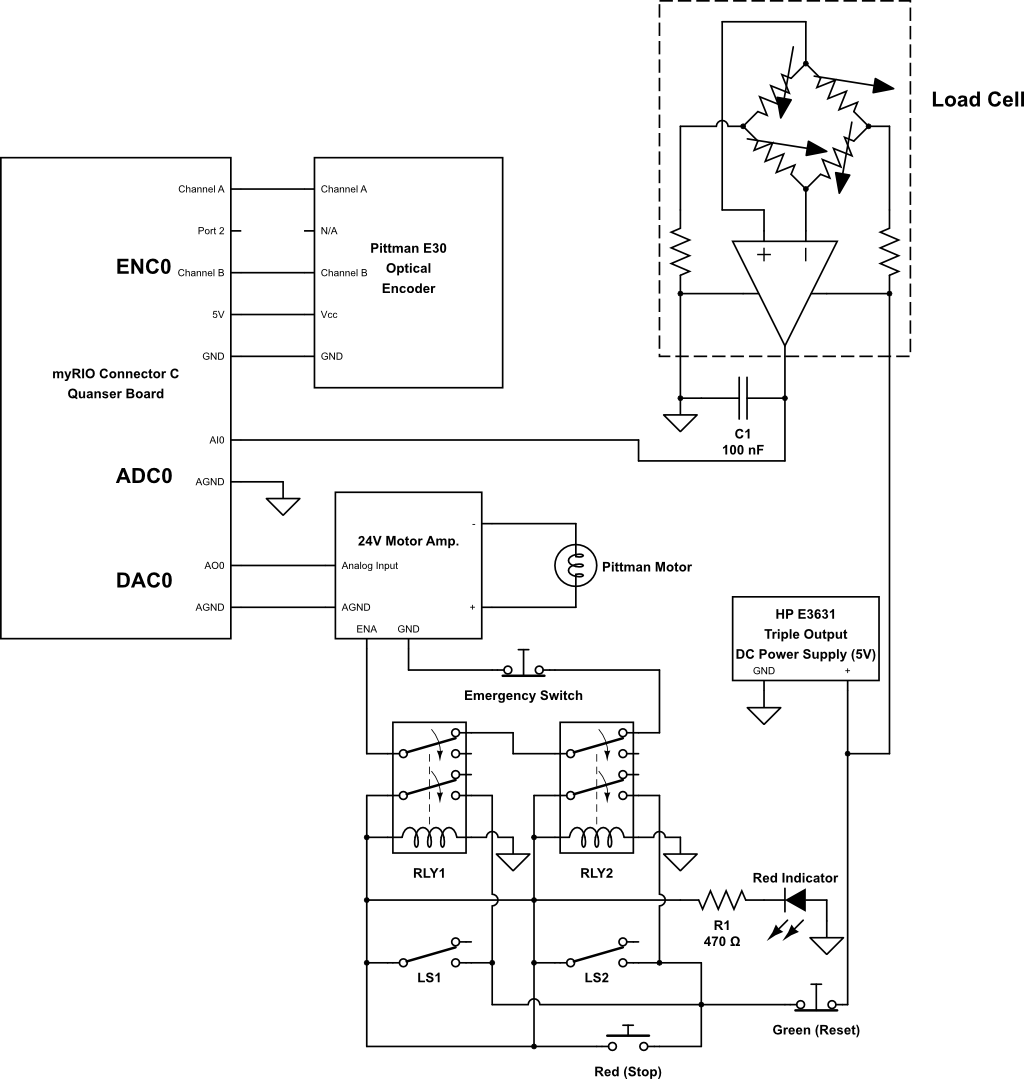
\includegraphics[width=2.75in]{Images/system_wiring_schematics.png}
    \caption{System Wiring Schematics}
    \label{SWS}
    \end{center}
    \end{figure}
%---Encoder Wiring
    \item{Encoder Wiring:}\par
    Figure \ref{EWS} shows the wiring of the input port in the quanser board to the output port of the E30 encoder, which is connected through a DIN connector.
    \begin{figure}[H]
    \begin{center}
    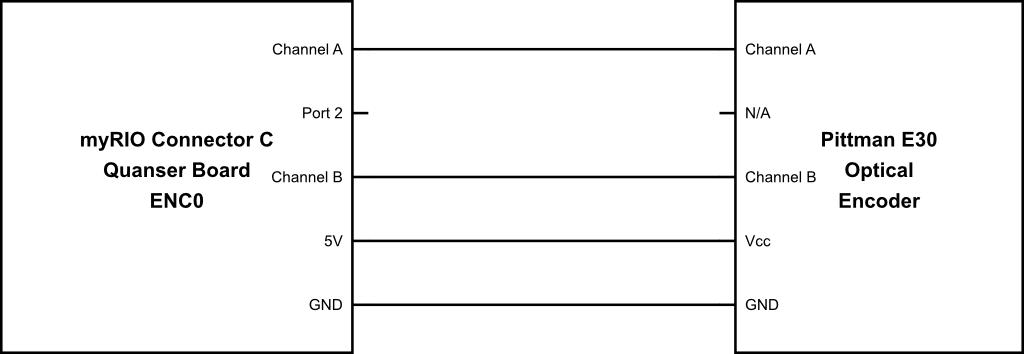
\includegraphics[width=2.75in]{Images/encoder_wiring.png}
    \caption{Encoder Wiring Schematics}
    \label{EWS}
    \end{center}
    \end{figure}
%---Motor Wiring
    \item{Motor Wiring Schematics:}\par
    Figure \ref{MWS} shows the wiring of the DAC output of the myRIO quanser board to the input of the 24V Motor Amplifier using a BNC connector. It also shows the connection between the motor itself and the 24V amplifier.
    \begin{figure}[H]
    \begin{center}
    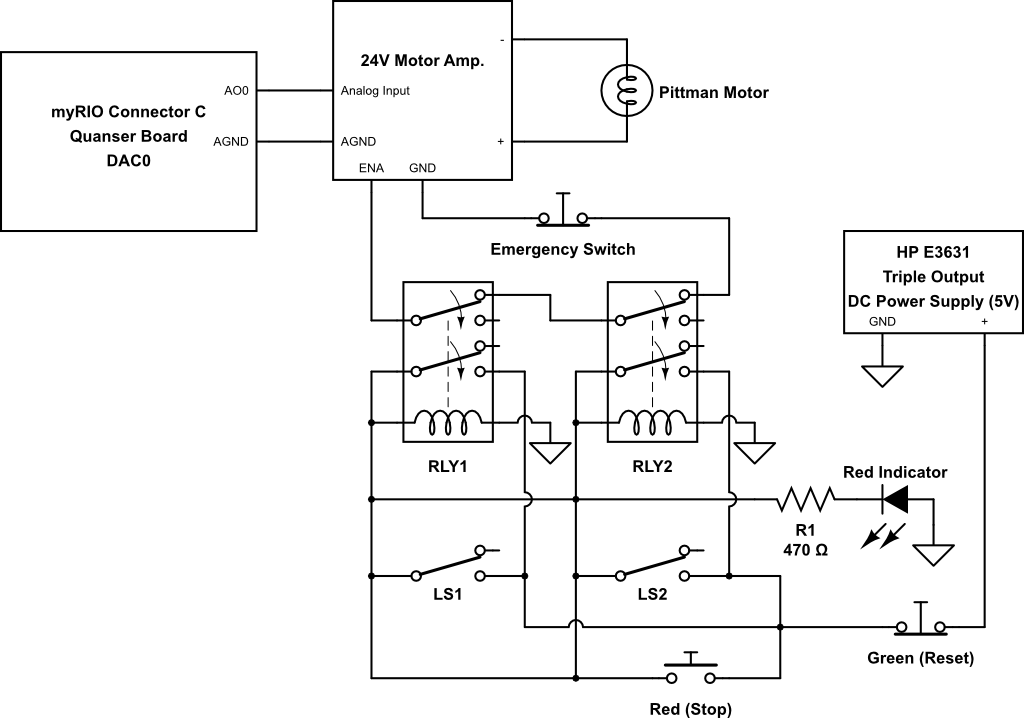
\includegraphics[width=2.75in]{Images/motor_wiring_wLS_circuit.png}
    \caption{Motor Wiring Schematics}
    \label{MWS}
    \end{center}
    \end{figure}
%---Limit Switch Wiring
    \item{Limit Switch Wiring Schematics:}\par
    Figure \ref{LSWS} shows a closer view of the wiring schematics of the limit switches to the electromechanical relays, which is supplied by the same HP E3631 DC power supply that is supplying the load cell. It also shows a closer view of the ``ENABLE'' circuit and how either one of the relays or the emergency switch will be able to open the circuit.
    \begin{figure}[H]
    \begin{center}
    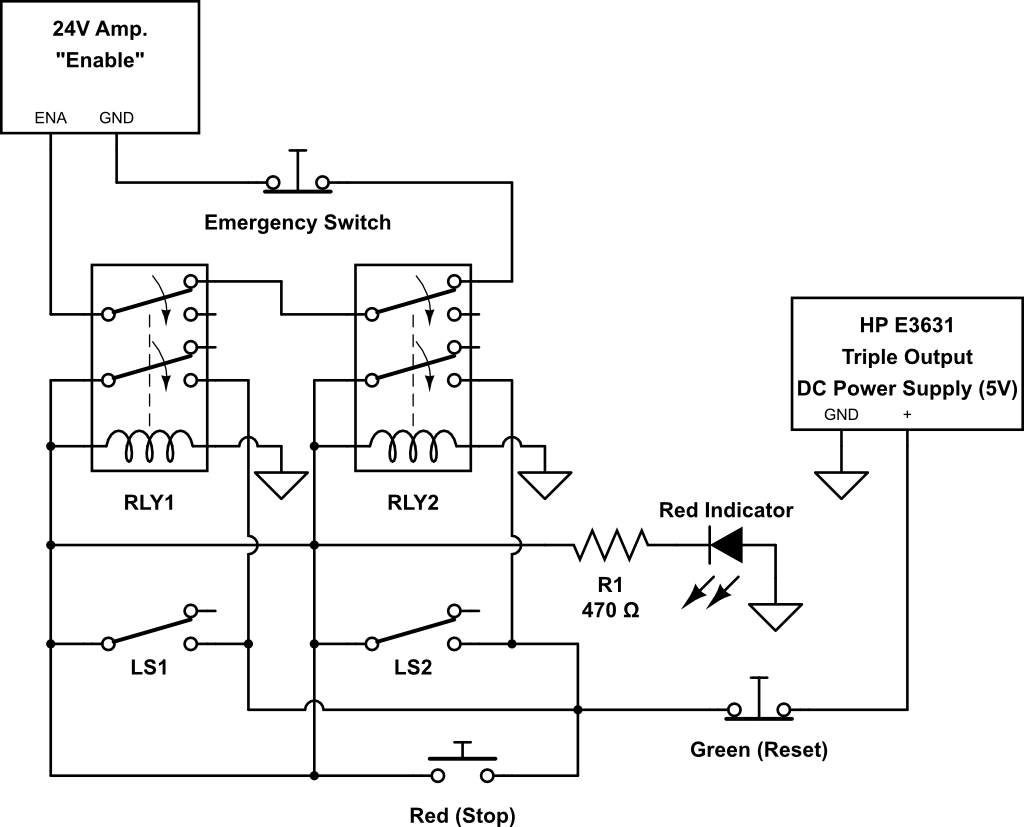
\includegraphics[width=2.75in]{Images/limit_switch_wiring.png}
    \caption{Limit Switch Wiring Schematics}
    \label{LSWS}
    \end{center}
    \end{figure}    
%---Load Cell Wiring
    \item{Load Cell Wiring Schematics:}\par
    Figure \ref{LCWS} shows the wiring of the load cell which is also supplied by the HP E3631 that is powering the relays. The figure also shows the output of the load cell being connected to a capacitor first, before connecting it to the ADC input of the myRIO quanser board in order to reduce the noise in the output signal.
    \begin{figure}[H]
    \begin{center}
    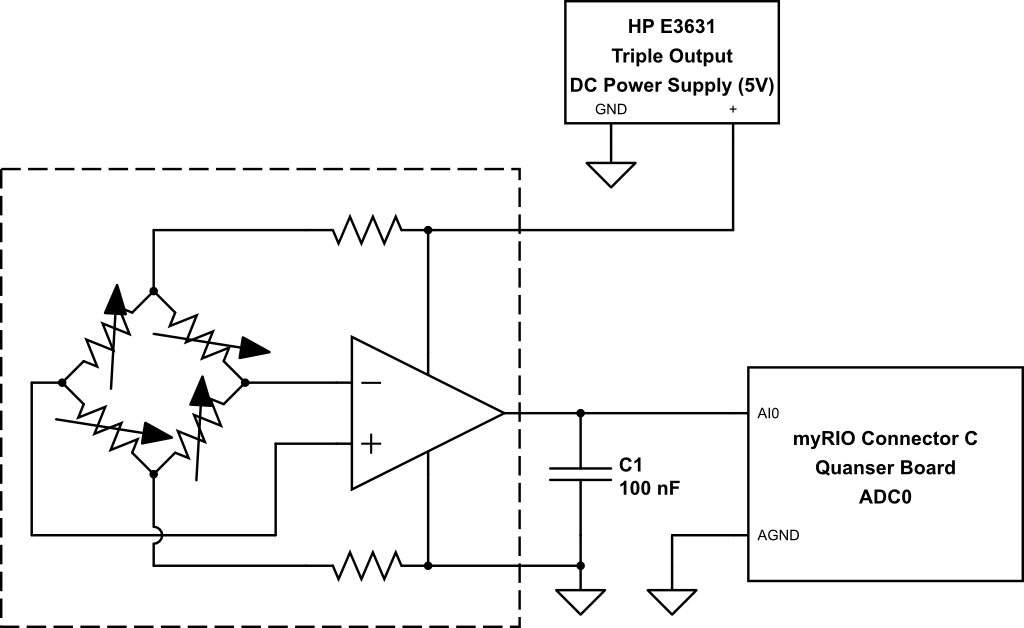
\includegraphics[width=2.75in]{Images/load_cell_wiring.png}
    \caption{Load Cell Wiring Schematics}
    \label{LCWS}
    \end{center}
    \end{figure}
\end{enumerate}